\documentclass[aspectratio=169, 10pt]{beamer}

% --------------------------------------------------
% 中文與字型設定 (xeCJK for XeLaTeX)
% --------------------------------------------------
\usepackage{xeCJK}
\setCJKmainfont{Microsoft JhengHei}
\setCJKsansfont{Microsoft JhengHei}
\setCJKmonofont{KaiTi}

% --------------------------------------------------
% 延伸套件
% --------------------------------------------------
\usepackage{booktabs}
\usepackage{multicol}
\usepackage{amsmath, amssymb, amsfonts}
\usepackage{graphicx}
\usepackage{tikz}
\usetikzlibrary{positioning, arrows.meta, shapes.geometric, fit, backgrounds, shadows}
\usepackage{tabularx}
\usepackage{array}
\usepackage{tcolorbox}
\usepackage{caption}
\usepackage{appendixnumberbeamer}

% --------------------------------------------------
% 載入臺大 NTU 官方主題規範 (beamerthementu.sty)
% --------------------------------------------------
\usetheme{ntu}

% 設定配色：台大藍 (ntublue) 主主題色 + 台大金 (ntugold) 輔助色
\setcolor[ntugold]{ntublue}
\setdarkframecolor{darkthemepurple!20!black}

% 設定完整科系全銜 (嚴禁使用簡稱)
\setdepartment{國立臺灣大學 工學院 工程科學及海洋工程學系 智慧計算與網路實驗室 (iCAN Lab)}

% 自訂高亮色彩
\definecolor{HighlightRed}{HTML}{C00000}

% --------------------------------------------------
% 論文基本資訊
% --------------------------------------------------
\title{\fontsize{22}{26}\selectfont\bfseries 應用知識圖注意力網路於食譜推薦之\\ 效能評估與可解釋性研究}
\subtitle{\small Performance Evaluation and Explainability Study of Knowledge Graph Attention Network for Recipe Recommendation}
\author{\small 研究生：廖健合 \quad (學號：R12525066)\\[0.15cm]指導教授：張瑞益 教授\\[0.15cm]iCAN 智慧計算與網路實驗室}
\setdepartment{國立臺灣大學 工學院 工程科學及海洋工程學系 iCAN 智慧計算與網路實驗室}
\date{}

% --------------------------------------------------
% 正文開始
% --------------------------------------------------
\begin{document}

% ==================================================
% Title Page (完整 2 頁式台大標準封面)
% ==================================================
\inserttitlepage

% ==================================================
% Outline
% ==================================================
\begin{frame}{簡報大綱 Outline}
  \tableofcontents
\end{frame}

% ==================================================
% Section 1: 研究背景與動機
% ==================================================
\section{研究背景與動機}

\begin{frame}{食譜平台的資訊過載需要更有依據的推薦}
  \begin{columns}[t]
    \begin{column}{0.48\textwidth}
      \begin{itemize}
        \item \alert{\textbf{海量食譜選擇困難}}：現代飲食線上平台包含數百萬筆食譜、食材組合與使用者互動數據，使用者難以快速定位符合個人偏好的餐點。
        \item \alert{\textbf{傳統推薦系統瓶頸}}：純協同過濾 (Collaborative Filtering, CF) 僅依賴使用者歷史點擊或評分，嚴重受限於數據稀疏性與冷啟動問題。
      \end{itemize}
    \end{column}
    
    \begin{column}{0.48\textwidth}
      \begin{itemize}
        \item \alert{\textbf{知識圖 (KG) 注入}}：將食譜、食材與標籤構建為協同知識圖，可豐富輔助語意並實現跨項目推理。
        \item \alert{\textbf{研究核心疑問}}：知識圖注意力網路 (KGAT) 在食譜推薦上的真正效能增益為何？由注意力權重導出的解釋路徑，是否能忠實反映模型的實際決策？
      \end{itemize}
    \end{column}
  \end{columns}
  
  \vspace{0.2cm}
  \begin{mybox}{ntublue}{研究核心目標}
    本研究旨在針對 \textbf{KGAT 在食譜推薦場景}進行實證評估，系統性量化傳播深度與知識圖整合對推薦效能及訓練行為之影響，並以 Fidelity 量化指標檢驗由注意力權重所萃取之解釋路徑忠實度 (Explanation Fidelity)。
  \end{mybox}
\end{frame}

\begin{frame}{協同知識圖 (CKG) 在食譜場景的建構}
  \begin{columns}[t]
    \begin{column}{0.5\textwidth}
      \begin{itemize}
        \item \alert{\textbf{使用者--食譜互動圖}} $\mathcal{G}_1$：
          包含使用者 $u \in \mathcal{U}$ 對食譜 $i \in \mathcal{I}$ 的歷史互動數據。
        \item \alert{\textbf{食譜知識圖}} $\mathcal{G}_2$：
          包含三元組 $(h, r, t) \in \mathcal{G}_2$，例如：
          \begin{itemize}
            \item (食譜 A, \textit{has\_ingredient}, 雞胸肉)
            \item (食譜 A, \textit{has\_tag}, 低碳水化合物)
          \end{itemize}
        \item \alert{\textbf{統一 CKG 架構}} $\mathcal{G} = \mathcal{G}_1 \cup \mathcal{G}_2$：
          將互動圖與知識圖融合為統一的異質圖結構。
      \end{itemize}
    \end{column}

    \begin{column}{0.46\textwidth}
      \begin{examplebox}{CKG 異質圖示意結構}
        \centering
        \begin{tikzpicture}[node distance=1.1cm, every node/.style={circle, draw=ntublue!80, fill=ntublue!10, inner sep=2pt, font=\tiny\bfseries}]
          \node (u1) [fill=ntugold!30, draw=ntugold!90] {User};
          \node (r1) [right=1.2cm of u1] {Recipe 1};
          \node (i1) [above right=0.7cm and 1.6cm of r1, fill=green!20, draw=green!60!black] {雞胸肉};
          \node (t1) [below right=0.7cm and 1.6cm of r1, fill=orange!20, draw=orange!60!black] {低卡};
          \node (r2) [below=1.2cm of r1] {Recipe 2};

          \draw[-{Stealth}, thick, ntublue] (u1) -- node[above, font=\tiny, draw=none, fill=none] {interact} (r1);
          \draw[-{Stealth}, thick, ntublue] (u1) -- (r2);
          \draw[-{Stealth}, dotted, thick] (r1) -- node[above left, pos=0.45, font=\tiny, draw=none, fill=none] {has\_ingredient} (i1);
          \draw[-{Stealth}, dotted, thick] (r1) -- node[below left, pos=0.45, font=\tiny, draw=none, fill=none] {has\_tag} (t1);
          \draw[-{Stealth}, dotted, thick] (r2) -- (t1);
        \end{tikzpicture}
      \end{examplebox}
    \end{column}
  \end{columns}
\end{frame}

% ==================================================
% Section 2: 文獻探討與問題定義
% ==================================================
\section{文獻探討與問題定義}

\begin{frame}{推薦模型演進與對比：從矩陣分解到圖神經網路}
  \begin{mybox}{ntublue}{}
    \small
    \setlength{\tabcolsep}{4pt}
    \renewcommand{\arraystretch}{0.9}
    \begin{tabularx}{\textwidth}{l X X X}
      \toprule
      \textbf{模型類別} & \textbf{代表方法} & \textbf{核心優勢 (Pros)} & \textbf{局限性 (Cons) / 本文缺口} \\
      \midrule
      \textbf{矩陣分解 (CF)} & BPR-MF & 運算簡單，擬合高頻互動 & 無法利用語意，冷啟動差 \\
      \midrule
      \textbf{特徵互動 (FM)} & NFM & 捕捉非線性高階特徵互動 & 視實體為獨立特徵，無視拓樸 \\
      \midrule
      \textbf{圖卷積 (GNN)} & LightGCN & 簡化 GNN，高效傳播訊號 & 僅處理單一關係，無視異質性 \\
      \midrule
      \textbf{圖注意力 (KGAT)} & \textbf{KGAT (本文)} & \textbf{融合 CKG 與注意力多跳傳播} & \textbf{既有研究缺乏食譜實證與解釋忠實度} \\
      \bottomrule
    \end{tabularx}
  \end{mybox}

  \vspace{0.12cm}
  \small \textbf{與食譜領域 KG 研究對比}：既有領域研究 (如 \textit{Li et al., JWS 2023}) 多專注於健康/營養之語意應用構建；本研究聚焦於 Food.com 協同知識圖中，\textbf{不同傳播深度對推薦效能與訓練行為的實證分析}，並以 Fidelity 檢驗\textbf{注意力導出解釋路徑之忠實度}。
\end{frame}

\begin{frame}{本研究解決的三大核心問題 (Research Questions)}
  \begin{columns}[t]
    \begin{column}{0.32\textwidth}
      \begin{mybox}[height=5.3cm]{ntublue}{{RQ1: 傳播深度與效能}}
        \small
        KGAT 在具備豐富食材與風味語意的 Food.com 食譜資料集上，不同傳播深度與知識圖整合，相較於頂尖基線 (LightGCN) 帶來何種排序表現影響？
      \end{mybox}
    \end{column}
    
    \begin{column}{0.32\textwidth}
      \begin{mybox}[height=5.3cm]{ntublue}{{RQ2: 訓練行為與早停}}
        \small
        不同傳播深度 ($L=1\sim 3$) 如何影響模型的訓練收斂動態與過擬合傾向？深層模型對早停機制 (Early Stopping) 的依賴為何？
      \end{mybox}
    \end{column}

    \begin{column}{0.32\textwidth}
      \begin{mybox}[height=5.3cm]{ntublue}{{RQ3: 注意力解釋忠實度}}
        \small
        基於注意力權重導出的候選解釋路徑，能否真實反映模型的實際決策？其解釋忠實度 (Explanation Fidelity) 指標 $F^+$ (必要性) 與 $F^-$ (充分性) 為何？
      \end{mybox}
    \end{column}
  \end{columns}
\end{frame}

% ==================================================
% Section 3: 研究方法 (KGAT 架構)
% ==================================================
\section{研究方法：KGAT 核心架構}

\begin{frame}{KGAT 模型整體架構示意圖}
  \vspace{-0.2cm}
  \makebox[\textwidth][c]{%
    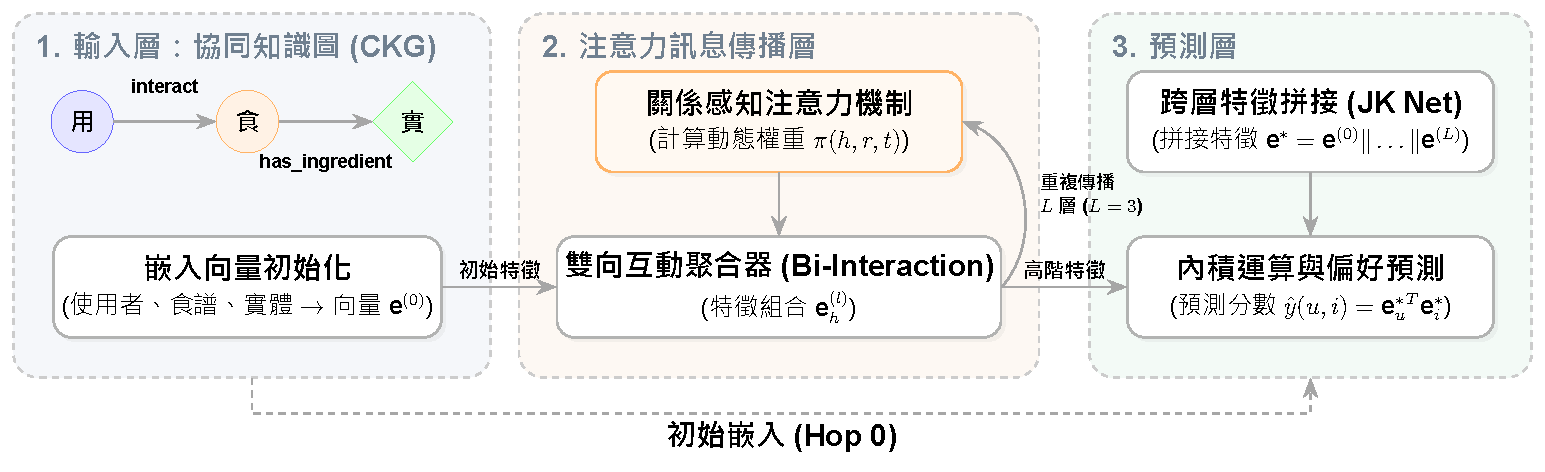
\includegraphics[width=1.12\textwidth, height=0.86\textheight, keepaspectratio]{../Main/figures/kgat_architecture.pdf}%
  }
\end{frame}

\begin{frame}{KGAT 核心模組一：關係感知注意力機制}
  \begin{itemize}
    \item \alert{\textbf{關係空間映射與原始分數 (Relation-aware Attention)}}：
      將實體 $h, t \in \mathcal{E}$ 與關係 $r \in \mathcal{R}$ 映射至關係空間，計算三元組原始相容性分數 $\pi(h, r, t)$：
      \[
        \pi(h, r, t) = (\mathbf{W}_r \mathbf{e}_t)^\top \tanh(\mathbf{W}_r \mathbf{e}_h + \mathbf{e}_r)
      \]
    \item \alert{\textbf{注意力 Softmax 歸一化權重}}：
      計算頭節點 $h$ 對其所有鄰居節點之歸一化注意力權重 $\alpha_{(h, r, t)}$：
      \[
        \alpha_{(h, r, t)} = \frac{\exp(\pi(h, r, t))}{\sum_{(h, r', t') \in \mathcal{N}_h} \exp(\pi(h, r', t'))}
      \]
  \end{itemize}

  \vspace{0.2cm}
  \begin{examplebox}{注意力機制特點}
    注意力權重 $\alpha_{(h, r, t)}$ 決定了訊息傳播時食材或標籤節點重要度，是後續萃取候選解釋路徑之關鍵權重依據。
  \end{examplebox}
\end{frame}

\begin{frame}{KGAT 核心模組二：雙重互動聚合與跨層拼接}
  \begin{itemize}
    \item \alert{\textbf{訊息聚合 (Information Aggregation)}}：
      計算實體 $h$ 在第 $l$ 層的一跳鄰居資訊表徵 $\mathbf{e}_{\mathcal{N}_h}^{(l)}$：
      \[
        \mathbf{e}_{\mathcal{N}_h}^{(l)} = \sum_{(h, r, t) \in \mathcal{N}_h} \alpha_{(h, r, t)} \mathbf{e}_t^{(l-1)}
      \]
    \item \alert{\textbf{雙重互動聚合器 (Bi-Interaction Aggregator)}}：
      同時捕捉加性累積與乘性過濾交互特徵：
      \[
        \mathbf{e}_h^{(l)} = \text{LeakyReLU}\Big( \mathbf{W}_1^{(l)} (\mathbf{e}_h^{(l-1)} + \mathbf{e}_{\mathcal{N}_h}^{(l)}) + \mathbf{W}_2^{(l)} (\mathbf{e}_h^{(l-1)} \odot \mathbf{e}_{\mathcal{N}_h}^{(l)}) \Big)
      \]
    \item \alert{\textbf{跨層拼接與預測 (Jumping Knowledge)}}：
      將 $0 \sim L$ 層特徵拼接獲得最終表徵 $\mathbf{e}_u^* = \mathbf{e}_u^{(0)} \| \dots \| \mathbf{e}_u^{(L)}$，預估推薦分數 $\hat{y}(u, i) = {\mathbf{e}_u^*}^T \mathbf{e}_i^*$。
  \end{itemize}
\end{frame}

\begin{frame}{損失函數：成對排序 BPR Loss 與模型優化}
  \begin{itemize}
    \item \alert{\textbf{Bayesian Personalized Ranking (BPR) Loss}}：
      鼓勵模型對使用者歷史互動過的正樣本食譜 $i^+$ 給予高於未互動負樣本 $i^-$ 的預測分數：
      \[
        \mathcal{L}_{\text{KGAT}} = \sum_{(u, i^+, i^-) \in \mathcal{D}} -\ln \sigma\Big(\hat{y}(u, i^+) - \hat{y}(u, i^-)\Big) + \lambda \|\mathbf{\Theta}\|_2^2
      \]
    \item \alert{\textbf{隨機負樣本抽樣與正則化}}：
      加入 $L_2$ 正則化項 ($\lambda=10^{-5}$) 避免嵌入向量過擬合，參數矩陣 $\mathbf{\Theta}$ 採用 Adam 優化器與 BFloat16 混合精度訓練。
  \end{itemize}
\end{frame}

% ==================================================
% Section 4: 實驗結果與討論
% ==================================================
\section{實驗結果與討論}

\begin{frame}{實驗資料集：Food.com 食譜協同圖}
  \begin{columns}[t]
    \begin{column}{0.48\textwidth}
      \begin{itemize}
        \item \alert{\textbf{資料集來源}}：Food.com 真實食譜與互動數據。
        \item \alert{\textbf{關聯實體}}：食譜、食材 (Ingredients)、標籤 (Tags)。
        \item \alert{\textbf{超級節點修剪 (Super-node Pruning)}}：
          \begin{itemize}
            \item 移除前 0.5\% 高頻食材 (61 個) 與通用調味料 (13 個)，兩者聯集共排除 74 個食材實體。
            \item 移除出現頻率前 50 個通用熱門標籤。
          \end{itemize}
      \end{itemize}
    \end{column}

    \begin{column}{0.48\textwidth}
      \begin{mybox}{ntublue}{Food.com CKG 統計規模}
        \small
        \begin{itemize}
          \item \textbf{使用者數量 $|\mathcal{U}|$}: 226,570
          \item \textbf{食譜數量 $|\mathcal{I}|$}: 231,637
          \item \textbf{歷史互動數}: 1,132,367
          \item \textbf{修剪後 KG 屬性實體}: 15,370
          \item \textbf{修剪後 KG 三元組}: 2,230,927
          \item \textbf{CKG 總邊數（含反向邊與自迴圈）}: \textbf{7,200,165}
        \end{itemize}
      \end{mybox}
    \end{column}
  \end{columns}
\end{frame}

% ==================================================
% P12: RQ1 效能評估 (大字體、清晰無擠壓)
% ==================================================
\begin{frame}{RQ1 效能評估：模型推薦表現長條圖對比}
  \begin{center}
    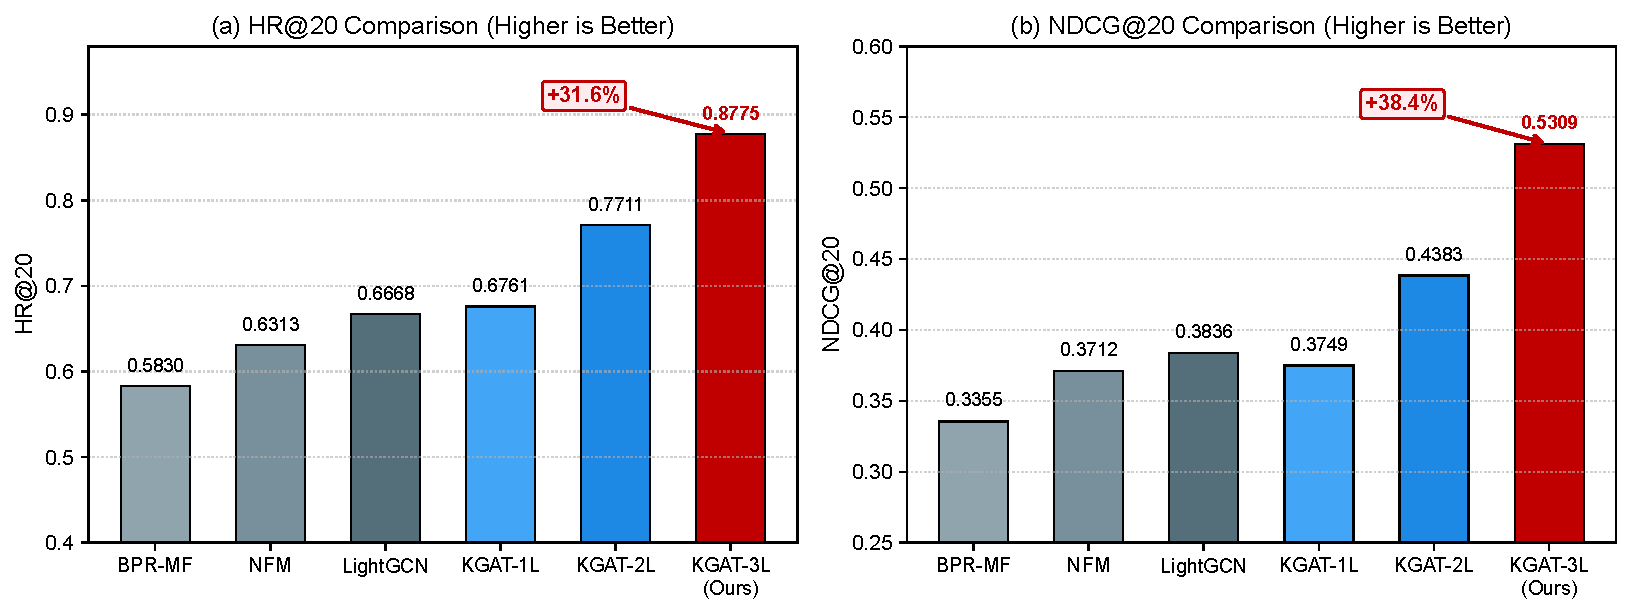
\includegraphics[width=0.92\linewidth, height=0.62\textheight, keepaspectratio]{../Main/figures/fig_performance_barchart.pdf}
  \end{center}

  \vspace{-0.15cm}
  \begin{alertblock}{\small\textbf{核心數據發現：KGAT-3L 推薦表現大幅超越強基線}}
    \small KGAT-3L 相較於最強圖卷積基線 LightGCN：\textbf{HR@20 相對提升 \textcolor{HighlightRed}{+31.6\%}} (0.6668 $\rightarrow$ \textbf{0.8775})，\textbf{NDCG@20 相對提升 \textcolor{HighlightRed}{+38.4\%}} (0.3836 $\rightarrow$ \textbf{0.5309})。(詳細數值表請見 附錄 A1/A2)
  \end{alertblock}
  \vspace{0.05cm}
  {\tiny *註：評估協定為 Leave-one-out 留一法搭配 100 個未互動負樣本排序，數值為三次獨立運行平均值。}
\end{frame}

% ==================================================
% P13: 淺層 KG 資訊污染 (標題特別醒目，內文精簡呈現實證數據)
% ==================================================
\begin{frame}{RQ1 多跳傳播層數與淺層 KG 資訊污染}
  \begin{columns}[t]
    \begin{column}{0.48\textwidth}
      \begin{itemize}
        \item \alert{\textbf{深度遞進效能 ($L=1\to 2\to 3$)}}：
          \begin{itemize}
            \item $L=1$ (0.6761) $\to L=2$ (0.7711, 較 1L +14.1\%) $\to L=3$ (\textbf{0.8775}, 較 1L +29.8\%, 較 2L +13.8\%)。
            \item 多跳傳播使模型能利用更高階圖拓撲資訊，且在本資料集上與效能提升呈現一致關聯。
          \end{itemize}
      \end{itemize}
    \end{column}

    \begin{column}{0.5\textwidth}
      \begin{alertblock}{\large\bfseries\color{HighlightRed} 發現：雜訊超越資訊增益，反而稀釋協同過濾訊號！}
        \small
        單跳傳播時高頻屬性節點灌注過度泛化特徵：\\[0.15cm]
        \textbf{實證數據}：\textbf{w/o KG-1L (0.7076)} 數值明顯高於 \mbox{\textbf{Full KGAT-1L (0.6761)}} 達 \textbf{\textcolor{HighlightRed}{+4.7\%}}！
      \end{alertblock}
      \vspace{0.15cm}
      \small \textbf{學術連結}：呼應 \textit{Zhang et al. (2025)} 關於「知識圖對推薦系統之貢獻非無條件正面」的實證觀察，亦可作為既有食譜 KG 研究 (如 \textit{Li et al., JWS 2023}) 採用複雜跨子圖機制的可能解釋之一。
    \end{column}
  \end{columns}
\end{frame}

% ==================================================
% P14: RQ2 訓練動態 (大字體表格)
% ==================================================
\begin{frame}{RQ2 訓練動態：各深度 Epoch 演變與早停機制}
  \begin{mybox}{ntublue}{不同深度模型前五個 Epoch 之 HR@20 演變趨勢 (三次獨立運行平均值)}
    \centering
    \vspace{0.1cm}
    \small
    \begin{tabular}{l c c c c c}
      \toprule
      \textbf{模型} & \textbf{Epoch 1} & \textbf{Epoch 2} & \textbf{Epoch 3} & \textbf{Epoch 4} & \textbf{Epoch 5} \\
      \midrule
      KGAT ($L=1$) & 0.6686 & 0.6690 & 0.6731 & 0.6728 & \textbf{0.6734} \\
      KGAT ($L=2$) & \textbf{0.7711} & 0.7645 & 0.7522 & 0.7455 & 0.7439 \\
      KGAT ($L=3$) & 0.8682 & \textbf{0.8696} & 0.8644 & 0.8496 & 0.8427 \\
      \bottomrule
    \end{tabular}
    \vspace{0.1cm}
  \end{mybox}

  \vspace{0.3cm}
  \begin{alertblock}{訓練行為結論：深層架構早停 (Early Stopping) 之必要性}
    淺層模型 ($L=1$) 參數量小且訓練平緩 (E5 達峰)；而深層模型 ($L=2, 3$) 具備廣大感受野，在 \textbf{Epoch 1～2 即迅速完成結構學習達效能峰值}，隨後測試效能下降可能反映深層模型的過擬合傾向；\textbf{因此實驗結果支持採用 Early Stopping，以降低後續 Epoch 的效能衰退風險}。
  \end{alertblock}
\end{frame}

% ==================================================
% P15: RQ2 訓練動態 (全頁大圖展示訓練與測試曲線)
% ==================================================
\begin{frame}{RQ2 訓練動態：訓練 Loss 與測試效能演變曲線}
  \begin{center}
    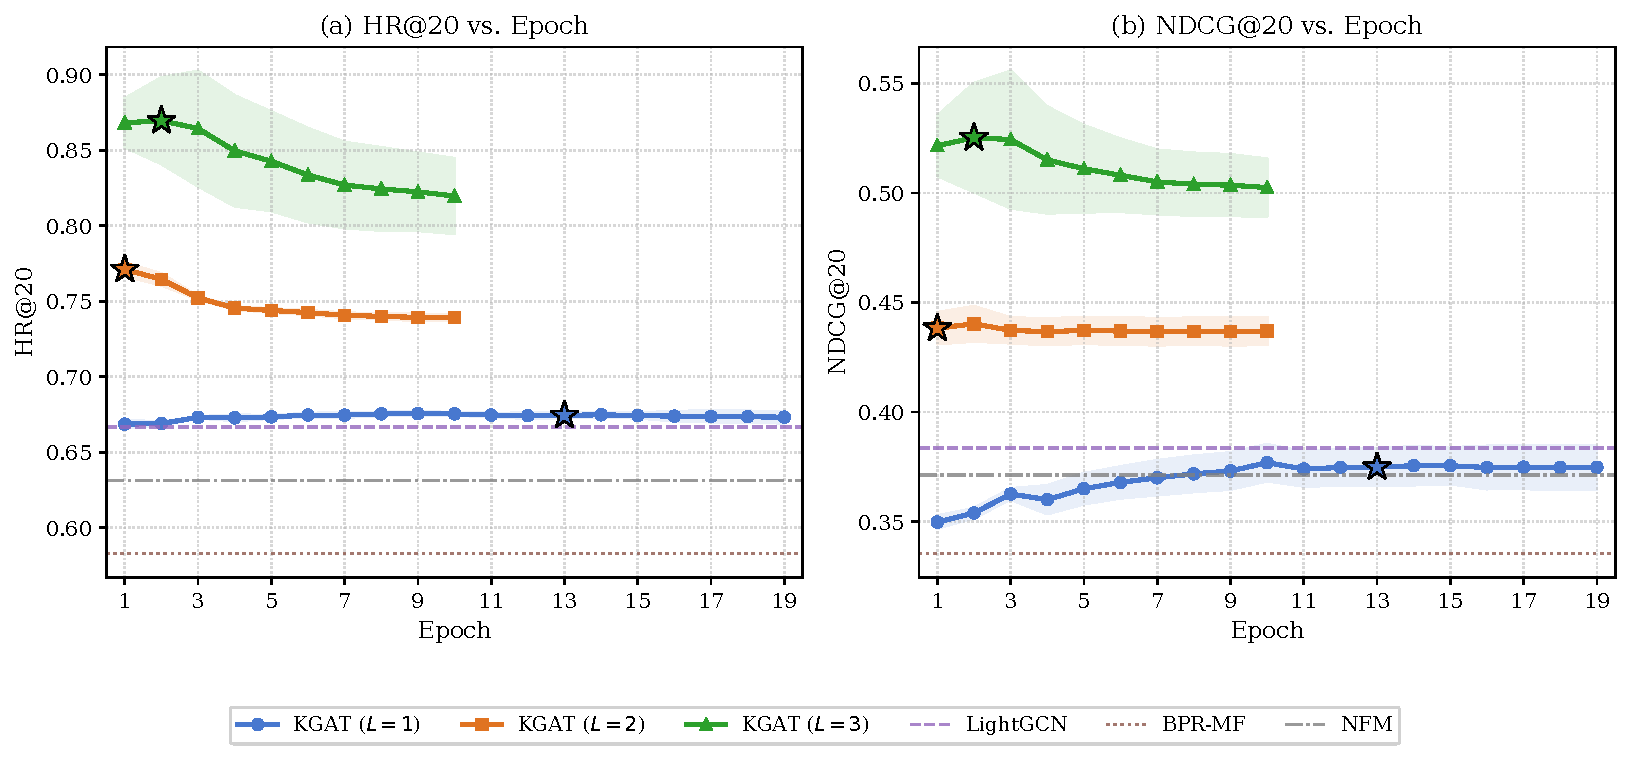
\includegraphics[width=0.92\linewidth, height=0.74\textheight, keepaspectratio]{../Main/figures/fig_training_curves.pdf}
  \end{center}
\end{frame}

\begin{frame}{RQ3 可解釋性分析：忠實度 (Fidelity) 評估機制}
  \begin{itemize}
    \item \alert{\textbf{正向忠實度 $F^+$ (Fidelity+ / 必要性)}}：
      從 CKG 中\textbf{移除} Top-$K$ 解釋子圖 $S$，觀察預測機率下降程度：
      \[
        F^+ = p_{uv} - p_{uv \setminus S} \quad (\text{若 } F^+ > 0 \text{ 代表該子圖邊為必要條件})
      \]
    \item \alert{\textbf{負向忠實度 $F^-$ (Fidelity- / 充分性)}}：
      遮蔽其餘邊，\textbf{僅保留} Top-$K$ 解釋子圖 $S$，觀察預測維持程度：
      \[
        F^- = p_{uv} - p_{uv | S} \quad (\text{若 } F^- \approx 0 \text{ 代表該子圖邊具充分資訊})
      \]
  \end{itemize}

  \vspace{0.2cm}
  \begin{mybox}{ntublue}{理想解釋性要求}
    若注意力導出之路徑具備客觀解釋忠實度，解釋子圖 $S$ 之 $F^+$ 應呈現明確正值（必要），且 $F^-$ 應保持極小落差（充分）。
  \end{mybox}
\end{frame}

\begin{frame}{RQ3 不同路徑類型對忠實度的影響}
  \begin{mybox}{ntublue}{{Fidelity 數據對比 ($n=278$ 位有效使用者，共 488 條解釋路徑)}}
    \centering
    \vspace{0.05cm}
    \footnotesize
    \setlength{\tabcolsep}{1.8pt}
    \begin{tabular}{l l c c c c}
      \toprule
      \textbf{路徑類型} & \textbf{拓樸結構} & \textbf{路徑數} & \textbf{人數} & \textbf{Avg $F^+$ ($\uparrow$)} & \textbf{Avg $F^-$ ($\downarrow$)} \\
      \midrule
      \textbf{直接連接} & User $\to$ Recipe & 84 條 (17.2\%) & 84 人 & \textbf{0.0494} & \textbf{-0.0004} \\
      \textbf{協同過濾} & User $\to$ Rec $\to$ User $\to$ Rec & 218 條 (44.7\%) & 101 人 & 0.0349 & 0.0134 \\
      \textbf{KG 語意} & User $\to$ Rec $\to$ Entity $\to$ Rec & 186 條 (38.1\%) & 93 人 & 0.0223 & \textbf{0.2449} \\
      \bottomrule
    \end{tabular}
    \vspace{0.05cm}
  \end{mybox}

  \vspace{0.15cm}
  \begin{alertblock}{重大發現：KG 語意路徑充分性偏低 ($F^- = 0.2449$)}
    「僅保留 KG 語意路徑」會造成約 24.5\% 的預測機率損失，支持一項可能解釋：知識圖的部分結構資訊可能在多層非線性傳播後被編碼至分散式嵌入中（本研究尚未直接驗證此機制），顯式路徑無法單獨涵蓋完整決策。
  \end{alertblock}
  \vspace{0.05cm}
  {\tiny *註：路徑佔比依 488 條路徑計算；Avg $F^+/F^-$ 依分組使用者計算。KGAT-3L 中 94.2\% (262/278 位有效使用者) 之 $F^+ > 0$。}
\end{frame}

% ==================================================
% P18: 嵌入 user_83279.pdf 圖檔與去標頭
% ==================================================
\begin{frame}{食譜推薦個案分析 Case C (User \#963993)}
  \begin{columns}[c]
    \begin{column}{0.54\textwidth}
      \centering
      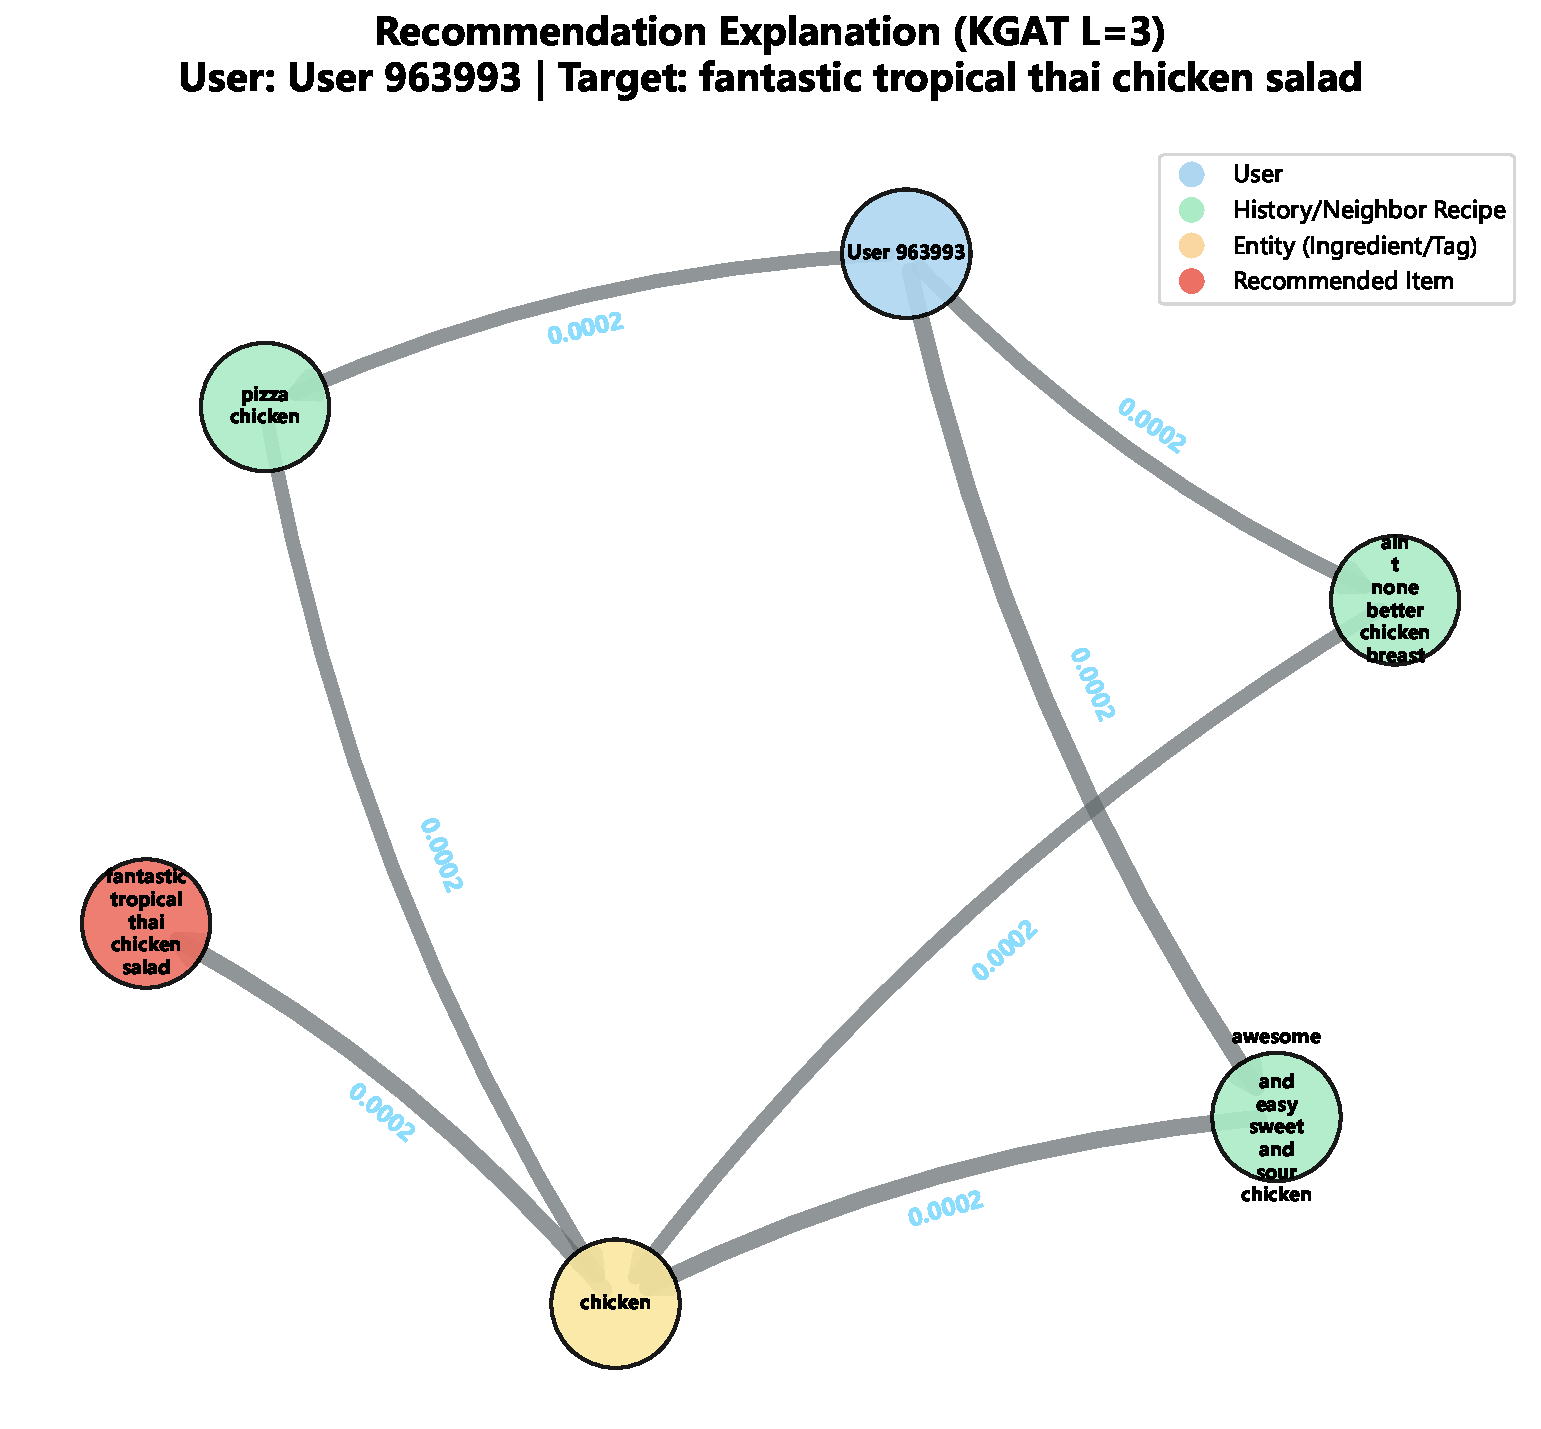
\includegraphics[width=\linewidth, height=0.72\textheight, keepaspectratio]{../Main/figures/user_83279.pdf}
    \end{column}

    \begin{column}{0.44\textwidth}
      \begin{mybox}{ntublue}{{Fidelity 評估數據與指標}}
        \small
        \begin{itemize}
          \item \textbf{推薦食譜}：\texttt{fantastic tropical thai chicken salad} (預測機率 0.933)
          \item \textbf{共同食材}：\texttt{chicken}
          \item \textbf{Fidelity 數據}：
            \begin{itemize}
              \item \textbf{$F^+ = -0.001$} (移除此路徑預測不降反升)
              \item \textbf{$F^- = 0.5415$} (僅留此路徑損失 54\% 機率)
            \end{itemize}
        \end{itemize}
      \end{mybox}
      \vspace{0.1cm}
      \small \textbf{案例啟示}：直觀語意合理 $\neq$ 忠實反映模型內部決策。
    \end{column}
  \end{columns}
\end{frame}

% ==================================================
% Section 5: 結論與未來展望
% ==================================================
\section{結論與未來展望}

\begin{frame}{論文主要貢獻總結}
  \begin{columns}[t]
    \begin{column}{0.32\textwidth}
      \begin{mybox}[fonttitle=\small\bfseries, height=5.0cm]{ntublue}{{貢獻一：傳播深度實證}}
        在 Food.com 食譜異質圖上系統性量化傳播深度，證實 KGAT-3L 達 0.8775 HR@20，相較強基線 LightGCN 展現大幅排序優勢 (+31.6\%)。
      \end{mybox}
    \end{column}

    \begin{column}{0.32\textwidth}
      \begin{mybox}[fonttitle=\small\bfseries, height=5.0cm]{ntublue}{{貢獻二：淺層 KG 污染現象}}
        揭示淺層 ($L=1$) 整合 KG 之條件式效能下降現象 (w/o KG 0.7076 > Full 0.6761)，對「外部知識必然改善推薦」的假設提出條件式質疑。
      \end{mybox}
    \end{column}

    \begin{column}{0.32\textwidth}
      \begin{mybox}[fonttitle=\small\bfseries, height=5.0cm]{ntublue}{{貢獻三：解釋路徑忠實度量化}}
        建立 $F^+ / F^-$ 擾動評估流程，實證注意力導出路徑之忠實度：直連與協同路徑具高忠實度，而 KG 語意路徑充分性偏低 ($F^- = 0.2449$)。
      \end{mybox}
    \end{column}
  \end{columns}
\end{frame}

\begin{frame}{未來研究方向}
  \vspace{-0.15cm}
  \begin{itemize}
    \setlength{\itemsep}{2pt}
    \item \alert{\textbf{擴展訓練規模與統計顯著性檢定}}
      \begin{itemize}\small
        \item 增加獨立重複執行次數（5 次以上），導入 paired $t$-test 與信心區間。
        \item 結合 DropEdge 與動態 Early Stopping，緩解深層圖網路過擬合。
      \end{itemize}

    \item \alert{\textbf{探究 KG 語意路徑充分性瓶頸}}
      \begin{itemize}\small
        \item 自圖資訊瓶頸 (GIB) 角度，解析多層傳播是否將部分結構資訊編碼至分散式嵌入中。
        \item 引入反事實 Fidelity 指標與路徑擾動管線，減緩邊遮罩引發之分佈偏移。
      \end{itemize}

    \item \alert{\textbf{跨領域多資料集與評估協定驗證}}
      \begin{itemize}\small
        \item 將淺層「資訊污染」現象推廣至 Amazon-Book、Yelp2018 跨領域圖譜驗證。
        \item 結合 Full-ranking 評估協定，檢驗抽樣條件對排序與指標絕對值之影響。
      \end{itemize}

    \item \alert{\textbf{消融實驗之系統性深層擴展}}
      \begin{itemize}\small
        \item 將模組拆解 (w/o Attention, w/o KG) 系統性拓展至 $L=2, 3$ 深層配置。
        \item 釐清注意力與知識圖在不同深度之邊際貢獻，建構完整元件貢獻圖像。
      \end{itemize}
  \end{itemize}
\end{frame}

{
  \def\insertsection{}
  \begin{frame}{}
    \begin{center}
      \vspace{0.8cm}
      {\Huge\bfseries\color{ntublue} 敬請 各位委員指導與賜教}\\[0.6cm]
      {\fontsize{18pt}{22pt}\selectfont\bfseries\color{ntugold} Thank You for Your Attention!}\\[1.4cm]
      \small 國立臺灣大學 工學院 工程科學及海洋工程學系 智慧計算與網路實驗室 (iCAN Lab)
    \end{center}
  \end{frame}
}

% ==================================================
% Section 6: 附錄 (Appendix)
% ==================================================
\appendix
\def\insertsection{附錄 (Appendix)}
\section*{附錄 (Appendix)}

\begin{frame}{附錄 A1: 基準模型與深度對比完整數據}
  \begin{mybox}{ntublue}{詳細對比表格 (三次獨立運行平均值)}
    \centering
    \resizebox{0.95\textwidth}{!}{%
    \begin{tabular}{l c c c c c c c c c}
      \toprule
      \textbf{Model} & \textbf{HR@10} & \textbf{HR@20} & \textbf{HR@50} & \textbf{NDCG@10} & \textbf{NDCG@20} & \textbf{NDCG@50} & \textbf{P@10} & \textbf{P@20} & \textbf{P@50} \\
      \midrule
      BPR-MF & 0.4683 & 0.5830 & 0.7416 & 0.3066 & 0.3355 & 0.3670 & 0.0468 & 0.0291 & 0.0148 \\
      NFM & 0.5108 & 0.6313 & 0.7946 & 0.3408 & 0.3712 & 0.4037 & 0.0511 & 0.0316 & 0.0159 \\
      LightGCN & 0.5320 & 0.6668 & 0.8516 & 0.3495 & 0.3836 & 0.4203 & 0.0532 & 0.0333 & 0.0170 \\
      \midrule
      KGAT-1L & 0.5483 & 0.6761 & 0.8366 & 0.3426 & 0.3749 & 0.4068 & 0.0548 & 0.0338 & 0.0167 \\
      KGAT-2L & 0.6219 & 0.7711 & 0.9464 & 0.4005 & 0.4383 & 0.4735 & 0.0622 & 0.0386 & 0.0189 \\
      \textbf{KGAT-3L} & \textbf{0.7348} & \textbf{0.8775} & \textbf{0.9830} & \textbf{0.4946} & \textbf{0.5309} & \textbf{0.5524} & \textbf{0.0735} & \textbf{0.0439} & \textbf{0.0197} \\
      \bottomrule
    \end{tabular}%
    }
  \end{mybox}
\end{frame}

\begin{frame}{附錄 A2: RQ1 模組消融實驗完整對比 (Ablation Study)}
  \begin{mybox}{ntublue}{模組消融評估數據 (三次獨立運行平均值)}
    \centering
    \resizebox{0.95\textwidth}{!}{%
    \begin{tabular}{l c c c c c c c c c}
      \toprule
      \textbf{實驗設定} & \textbf{HR@10} & \textbf{HR@20} & \textbf{HR@50} & \textbf{NDCG@10} & \textbf{NDCG@20} & \textbf{NDCG@50} & \textbf{P@10} & \textbf{P@20} & \textbf{P@50} \\
      \midrule
      Full KGAT ($L{=}1$) & 0.5483 & 0.6761 & 0.8366 & 0.3426 & 0.3749 & 0.4068 & 0.0548 & 0.0338 & 0.0167 \\
      w/o Attention ($L{=}1$) & 0.5483 & 0.6636 & 0.8081 & 0.3653 & 0.3945 & 0.4231 & 0.0548 & 0.0332 & 0.0162 \\
      w/o KG ($L{=}1$) & 0.5704 & 0.7076 & 0.8761 & 0.3768 & 0.4114 & 0.4450 & 0.0571 & 0.0354 & 0.0175 \\
      \midrule
      KGAT ($L{=}2$) & 0.6219 & 0.7711 & 0.9464 & 0.4005 & 0.4383 & 0.4735 & 0.0622 & 0.0386 & 0.0189 \\
      \textbf{KGAT ($L{=}3$)} & \textbf{0.7348} & \textbf{0.8775} & \textbf{0.9830} & \textbf{0.4946} & \textbf{0.5309} & \textbf{0.5524} & \textbf{0.0735} & \textbf{0.0439} & \textbf{0.0197} \\
      \bottomrule
    \end{tabular}%
    }
  \end{mybox}
  \vspace{0.15cm}
  \begin{alertblock}{\small 關鍵發現與消融啟示}
    \footnotesize
    \begin{itemize}
      \item \textbf{w/o Attention ($L=1$)}：HR@20 略降 1.8\%，但均勻聚合具隱含正則化使 NDCG@20 略升 5.2\%；目前僅在 $L{=}1$ 觀察到均勻聚合對 HR@20 影響有限，注意力機制在 $L\ge 2$ 的邊際效益仍待後續消融實驗驗證。
      \item \textbf{w/o KG ($L=1$)}：退化為純二分圖反而使 HR@20 提升 4.7\%，顯示即使經過超級節點修剪，淺層 KG 中殘留的高連接度資訊仍可能稀釋協同過濾訊號。
    \end{itemize}
  \end{alertblock}
\end{frame}

\begin{frame}{附錄 B1: 食材 (Ingredients) 噪音過濾清單}
  \begin{mybox}{ntublue}{基礎調味料噪音清單 (Base Noise - 13 個實體)}
    \small \texttt{salt, water, oil, sugar, all-purpose flour, butter, eggs, black pepper, garlic, onions, vanilla, baking soda, baking powder}
  \end{mybox}
  
  \vspace{0.1cm}
  \begin{examplebox}{高頻食材過濾清單 (Top 0.5\% - 61 個實體)}
    \tiny
    \texttt{carrot, red onion, unsalted butter, green onion, zucchini, ground beef, ground cinnamon, honey, cream cheese, mayonnaise, fresh parsley, potatoes, celery, red bell pepper, tomatoes, dijon mustard, orange juice, cayenne pepper, margarine, olive oil, soy sauce, dried oregano, vegetable oil, garlic powder, worcestershire sauce, flour, powdered sugar, paprika, lemon juice, kosher salt, cheddar cheese, milk, sour cream, chili powder, nutmeg, fresh lemon juice, fresh ground black pepper, mozzarella cheese, cornstarch, parmesan cheese, heavy cream, chicken broth, raisins, granulated sugar, brown sugar, vanilla extract, extra virgin olive oil, bacon, walnuts, pecans, salt and pepper, ground cumin, pepper, egg}
  \end{examplebox}
\end{frame}

\begin{frame}{附錄 B2: 標籤 (Tags) 噪音過濾清單}
  \begin{mybox}{ntublue}{高頻過濾標籤清單 (Top 50 實體 - 共 552 個類別)}
    \tiny
    \texttt{4-hours-or-less, course, 15-minutes-or-less, comfort-food, desserts, oven, time-to-make, lunch, occasion, equipment, dietary, low-saturated-fat, preparation, holiday-event, healthy-2, low-carb, inexpensive, poultry, north-american, side-dishes, 3-steps-or-less, low-fat, vegetables, 5-ingredients-or-less, taste-mood, easy, 30-minutes-or-less, 60-minutes-or-less, european, low-sodium, low-cholesterol, low-protein, eggs-dairy, pasta-rice-and-grains, presentation, vegetarian, dinner-party, beginner-cook, fruit, kid-friendly, low-in-something, american, main-ingredient, for-1-or-2, healthy, low-calorie, main-dish, cuisine, number-of-servings, meat}
  \end{mybox}

  \vspace{0.15cm}
  \begin{alertblock}{論文附錄 C 修剪動機與結論}
    過濾 74 個高頻與通用食材 (61 個高頻 + 13 個通用) 與前 50 個熱門標籤，旨在防止超級節點 (Hub Nodes) 將高度同質化的資訊無差別廣播給大量不相關食譜，避免協同過濾訊號被稀釋，維繫語意鑑別度。
  \end{alertblock}
\end{frame}

\begin{frame}{附錄 C: 實驗超參數配置}
  \begin{mybox}{ntublue}{實驗統一超參數配置}
    \small
    \begin{itemize}
      \item \textbf{Embedding Dimension}: $d = 64$
      \item \textbf{Batch Size}: 1024 | \textbf{Learning Rate}: $\eta = 0.001$ (Adam Optimizer, StepLR)
      \item \textbf{L2 Regularization $\lambda$}: $10^{-5}$
      \item \textbf{訓練精度與硬體}: BFloat16 混合精度，Intel Arc A750 GPU (XPU)
      \item \textbf{評估協定}: Leave-one-out 留一法，正樣本搭配 100 個未互動負樣本
    \end{itemize}
  \end{mybox}
\end{frame}

\begin{frame}{附錄 D1: Case A 直接連接個案 (User \#2410864)}
  \begin{columns}[c]
    \begin{column}{0.54\textwidth}
      \centering
      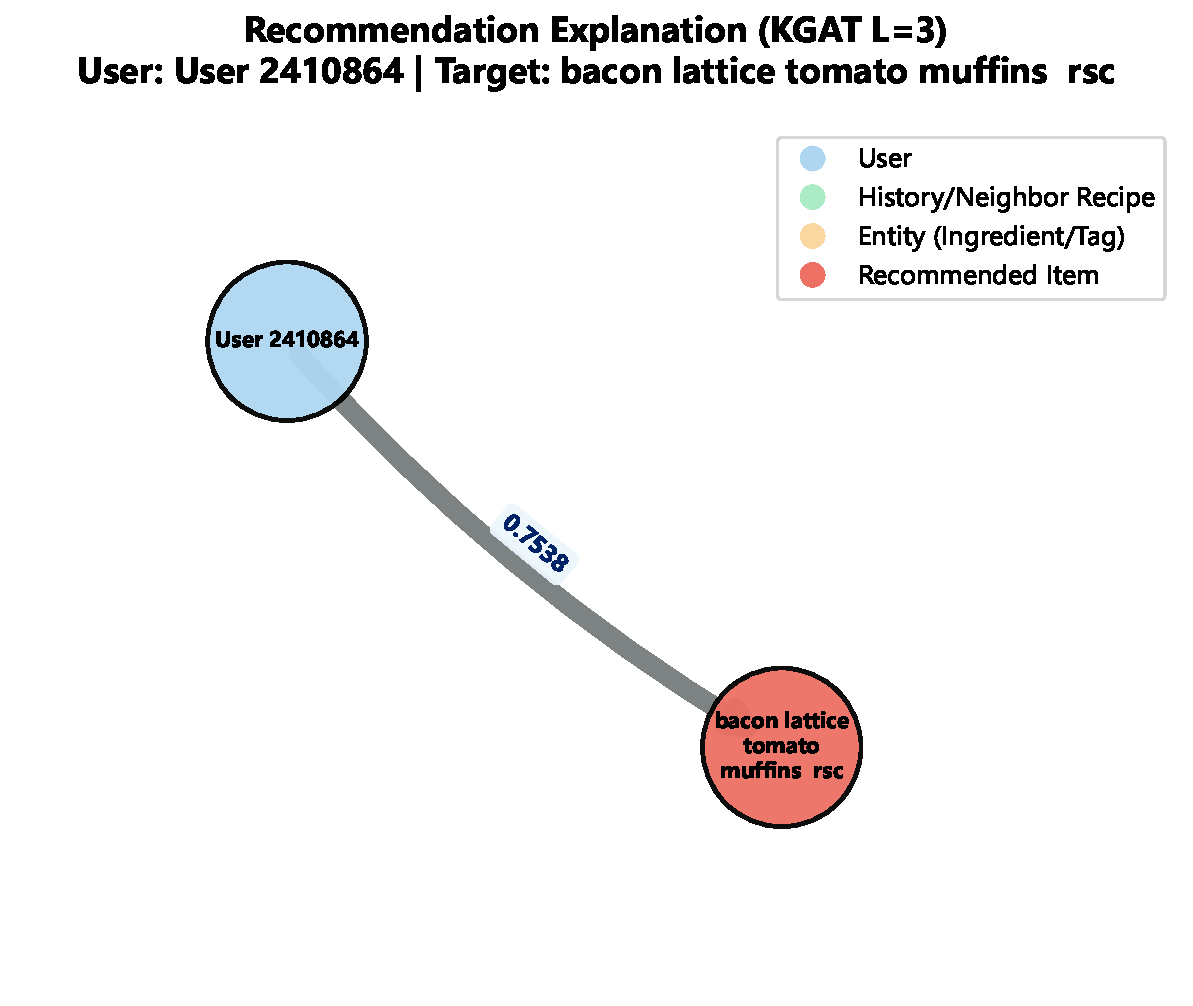
\includegraphics[width=\linewidth, height=0.70\textheight, keepaspectratio]{../Main/figures/user_141540.pdf}
    \end{column}

    \begin{column}{0.44\textwidth}
      \begin{mybox}{ntublue}{{Fidelity 評估數據與指標}}
        \footnotesize
        \begin{itemize}
          \item \textbf{推薦食譜}：\texttt{bacon lattice tomato muffins} (預測機率 0.952)
          \item \textbf{路徑類型}：Direct Link (User $\to$ Recipe)
          \item \textbf{注意力權重}：$\alpha = 0.767$
          \item \textbf{Fidelity 數據}：
            \begin{itemize}
              \item \textbf{$F^+ = 0.2415$} (\textbf{高必要性}，移除預測降 24\%)
              \item \textbf{$F^- = 0.0004$} (\textbf{接近 0}，僅留此邊維繫機率)
            \end{itemize}
          \item \textbf{案例判讀}：極高必要性與充分性。
        \end{itemize}
      \end{mybox}
    \end{column}
  \end{columns}
\end{frame}

\begin{frame}{附錄 D2: Case B 協同過濾個案 (User \#573230)}
  \begin{columns}[c]
    \begin{column}{0.54\textwidth}
      \centering
      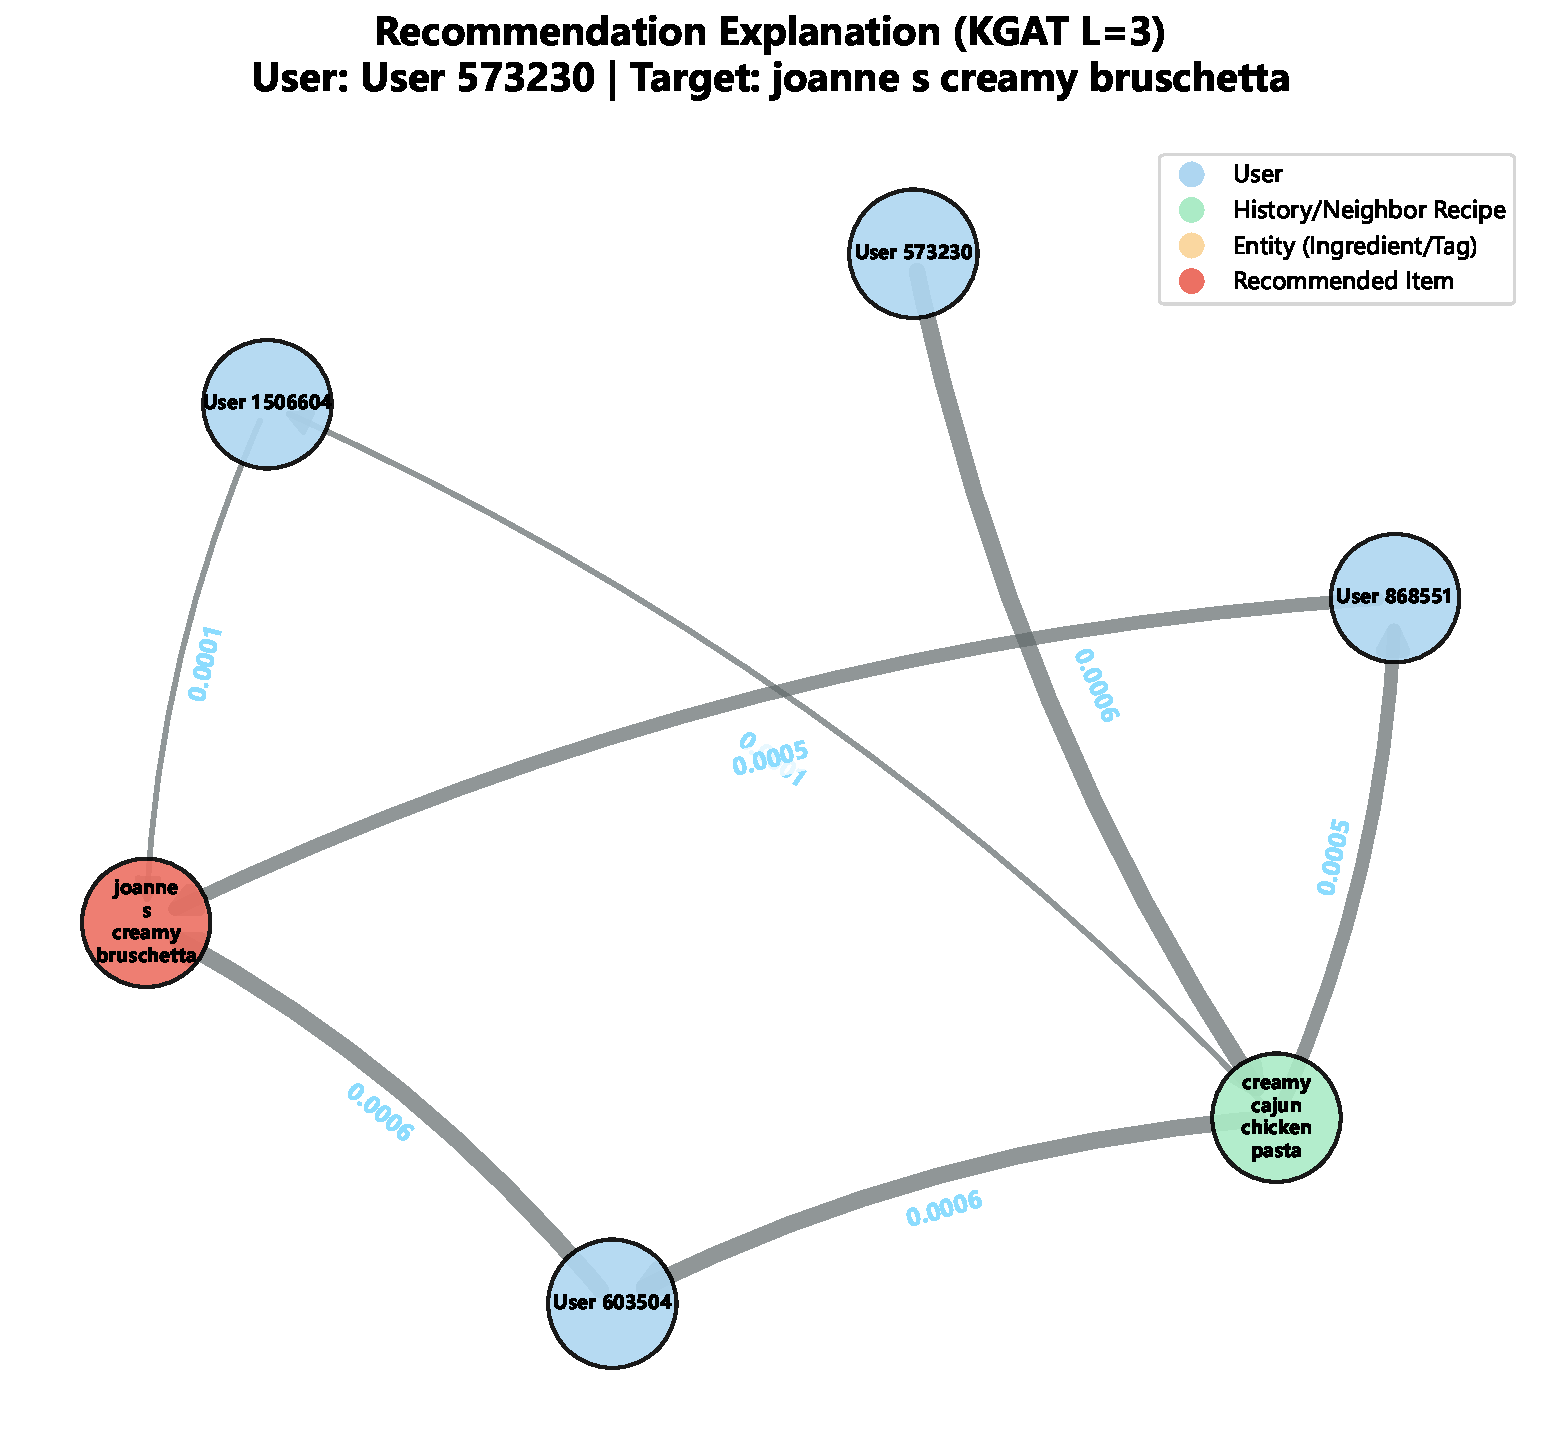
\includegraphics[width=\linewidth, height=0.74\textheight, keepaspectratio]{../Main/figures/user_58074.pdf}
    \end{column}

    \begin{column}{0.44\textwidth}
      \begin{mybox}{ntublue}{{Fidelity 評估數據與指標}}
        \small
        \begin{itemize}
          \item \textbf{推薦食譜}：\texttt{joanne's creamy bruschetta} (預測機率 0.952)
          \item \textbf{路徑類型}：CF Path (User $\to$ Rec $\to$ User $\to$ Rec)
          \item \textbf{Fidelity 數據}：
            \begin{itemize}
              \item \textbf{$F^+ = 0.2061$} (\textbf{高必要性}，移除預測降 20\%)
              \item \textbf{$F^- = 0.0019$} (\textbf{接近 0}，具備高充分性)
            \end{itemize}
          \item \textbf{案例判讀}：長路徑具良好忠實度。
        \end{itemize}
      \end{mybox}
    \end{column}
  \end{columns}
\end{frame}

\begin{frame}{附錄 E: Fidelity 方法限制與圖結構分佈偏移}
  \begin{itemize}
    \item \alert{\textbf{分佈偏移 (Distribution Shift)}}：
      當從圖中直接移除邊 ($F^+$) 或僅保留子圖 ($F^-$) 時，輸入特徵圖之拓樸結構發生突變，可能使模型進入訓練時未曾見過的狀態，導致 $F^-$ 評估出現偏高誤差（即 KG 語意路徑 $F^- = 0.2449$ 可能部分來自模型適應不良）。未來宜結合重訓練式或反事實評估。
  \end{itemize}
\end{frame}

\begin{frame}{附錄 F: 食譜 KG 指標性文獻 (Li et al., JWS 2023) 對比與定位}
  \begin{mybox}{ntublue}{{食譜 KG 指標性文獻對比 (Li et al., JWS 2023 vs. 本論文)}}
    \scriptsize
    \setlength{\tabcolsep}{2.5pt}
    \renewcommand{\arraystretch}{0.80}
    \begin{tabularx}{\textwidth}{l X X}
      \toprule
      \textbf{對比面向} & \textbf{Li et al. (JWS 2023)} & \textbf{本論文 (KGAT on Food.com)} \\
      \midrule
      \textbf{核心目標} & 高層健康語意引導與健康食譜推薦 & 評估 KGAT 效能增益、訓練動態與解釋忠實度 \\
      \midrule
      \textbf{知識圖譜} & 著重營養、健康屬性與專家語意圖譜 & 融合 Food.com 食材與標籤之 CKG (>720萬邊) \\
      \midrule
      \textbf{網絡架構} & 語意導向推薦與專家規則結合架構 & 關係感知注意力與雙重互動多跳傳播 ($L=1\sim3$) \\
      \midrule
      \textbf{關鍵貢獻} & 開創食譜語意網與健康推薦框架 & 揭示淺層資訊污染現象，量化注意力解釋忠實度 ($F^-=0.2449$) \\
      \bottomrule
    \end{tabularx}
  \end{mybox}

  \vspace{-0.35cm}
  \begin{alertblock}{\small 本論文於學術脈絡之定位與互補性}
    \footnotesize
    Li et al. (JWS 2023) 著重於\textbf{高層健康語意與領域知識}整合，而本論文著重於\textbf{不同傳播深度之實證比較與解釋路徑忠實度評估}。本研究在 Food.com 食譜推薦場景下，提供了淺層 KG 整合效果與注意力導出解釋路徑忠實度的實證分析（如 $F^- = 0.2449$ 暗示顯式路徑充分性不足）。
  \end{alertblock}
\end{frame}

\end{document}
